\subsection{XRD}
\begin{figure}[h!]
	\centering
	\centering
\begin{tikzpicture}[scale=0.9, rotate=-90]
	%\begin{sideways}
	\begin{axis}[
	scale only axis,
	ymode=log, 
	width=\textheight, 
	height=\textwidth %7cm
]
	\addplot [smooth,mark=*,black] table {%  plot X versus Y. This is original data.
	X		Y 
	
  0.595 545825
  0.605 652541
  0.615 643846
  0.625 655290
  0.635 654805
  0.645 638561
  0.655 639840
  0.665 549526
  0.675 515380
  0.685 394384
  0.695 362524
  0.705 280476
  0.715 257150
  0.725 210497
  0.735 199362
  0.745 166138
  0.755 153899
  0.765 128737
  0.775 123552
  0.785 106602
  0.795 100997
  0.805 83868
  0.815 76895
  0.825 67236
  0.835 66564
  0.845 60123
  0.855 57073
  0.865 48532
  0.875 43139
  0.885 37481
  0.895 37791
  0.905 36787
  0.915 36328
  0.925 32005
  0.935 27490
  0.945 22801
  0.955 21112
  0.965 21550
  0.975 22560
  0.985 22261
  0.995 20564
  1.005 17450
  1.015 14161
  1.025 12477
  1.035 12544
  1.045 13924
  1.055 14860
  1.065 15006
  1.075 12882
  1.085 10733
  1.095 8317
  1.105 7621
  1.115 8172
  1.125 9351
  1.135 10140
  1.145 10262
  1.155 8593
  1.165 7362
  1.175 5432
  1.185 5027
  1.195 5069
  1.205 6288
  1.215 7259
  1.225 7868
  1.235 6856
  1.245 5852
  1.255 4186
  1.265 3387
  1.275 3249
  1.285 4382
  1.295 4998
  1.305 5975
  1.315 5580
  1.325 5112
  1.335 3672
  1.345 2894
  1.355 2285
  1.365 2746
  1.375 3352
  1.385 4476
  1.395 4679
  1.405 4462
  1.415 3516
  1.425 2725
  1.435 1840
  1.445 1866
  1.455 2134
  1.465 3036
  1.475 3446
  1.485 3931
  1.495 3341
  1.505 2756
  1.515 1884
  1.525 1475
  1.535 1303
  1.545 1823
  1.555 2343
  1.565 3102
  1.575 3003
  1.585 2862
  1.595 2200
  1.605 1624
  1.615 1089
  1.625 1102
  1.635 1362
  1.645 1971
  1.655 2314
  1.665 2601
  1.675 2266
  1.685 1892
  1.695 1260
  1.705 912
  1.715 829
  1.725 1211
  1.735 1616
  1.745 2079
  1.755 2116
  1.765 1945
  1.775 1459
  1.785 1116
  1.795 745
  1.805 713
  1.815 870
  1.825 1303
  1.835 1568
  1.845 1789
  1.855 1632
  1.865 1362
  1.875 973
  1.885 650
  1.895 497
  1.905 734
  1.915 1005
  1.925 1391
  1.935 1436
  1.945 1421
  1.955 1253
  1.965 847
  1.975 548
  1.985 475
  1.995 484
  2.005 784
  2.015 1069
  2.025 1274
  2.035 1260
  2.045 1069
  2.055 745
  2.065 534
  2.075 335
  2.085 458
  2.095 562
  2.105 864
  2.115 912
  2.125 1063
  2.135 930
  2.145 778
  2.155 484
  2.165 328
  2.175 276
  2.185 433
  2.195 620
  2.205 795
  2.215 882
  2.225 853
  2.235 718
  2.245 543
  2.255 313
  2.265 276
  2.275 324
  2.285 484
  2.295 650
  2.305 697
  2.315 734
  2.325 655
  2.335 502
  2.345 320
  2.355 246
  2.365 204
  2.375 328
  2.385 471
  2.395 590
  2.405 610
  2.415 610
  2.425 493
  2.435 350
  2.445 250
  2.455 180
  2.465 213
  2.475 324
  2.485 475
  2.495 524
  2.505 529
  2.515 484
  2.525 320
  2.535 219
  2.545 180
  2.555 172
  2.565 240
  2.575 365
  2.585 396
  2.595 454
  2.605 445
  2.615 380
  2.625 282
  2.635 172
  2.645 130
  2.655 169
  2.665 222
  2.675 331
  2.685 376
  2.695 380
  2.705 350
  2.715 256
  2.725 172
  2.735 114
  2.745 128
  2.755 164
  2.765 225
  2.775 303
  2.785 361
  2.795 342
  2.805 269
  2.815 231
  2.825 146
  2.835 86
  2.845 100
  2.855 161
  2.865 213
  2.875 272
  2.885 296
  2.895 266
  2.905 240
  2.915 174
  2.925 128
  2.935 94
  2.945 92
  2.955 151
  2.965 199
  2.975 228
  2.985 222
  2.995 262
  3.005 190
  3.015 154
  3.025 100
  3.035 85
  3.045 117
  3.055 132
  3.065 182
  3.075 225
  3.085 237
  3.095 204
  3.105 154
  3.115 110
  3.125 85
  3.135 72
  3.145 114
  3.155 128
  3.165 174
  3.175 190
  3.185 180
  3.195 149
  3.205 125
  3.215 100
  3.225 72
  3.235 72
  3.245 88
  3.255 125
  3.265 151
  3.275 166
  3.285 164
  3.295 144
  3.305 100
  3.315 72
  3.325 67
  3.335 71
  3.345 90
  3.355 121
  3.365 151
  3.375 169
  3.385 151
  3.395 108
  3.405 86
  3.415 53
  3.425 62
  3.435 48
  3.445 90
  3.455 106
  3.465 130
  3.475 149
  3.485 125
  3.495 90
  3.505 72
  3.515 64
  3.525 53
  3.535 74
  3.545 79
  3.555 117
  3.565 135
  3.575 117
  3.585 98
  3.595 79
  3.605 55
  3.615 37
  3.625 49
  3.635 61
  3.645 72
  3.655 94
  3.665 100
  3.675 86
  3.685 85
  3.695 56
  3.705 56
  3.715 44
  3.725 59
  3.735 61
  3.745 74
  3.755 98
  3.765 88
  3.775 67
  3.785 67
  3.795 50
  3.805 44
  3.815 38
  3.825 31
  3.835 50
  3.845 58
  3.855 83
  3.865 66
  3.875 52
  3.885 46
  3.895 37
  3.905 41
  3.915 35
  3.925 45
  3.935 44
  3.945 59
  3.955 76
  3.965 76
  3.975 64
  3.985 44
  3.995 25
  4.005 38
  4.015 28
  4.025 38
  4.035 53
  4.045 55
  4.055 66
  4.065 71
  4.075 64
  4.085 42
  4.095 32
  4.105 34
  4.115 38
  4.125 38
  4.135 41
  4.145 56
  4.155 50
  4.165 44
  4.175 35
  4.185 31
  4.195 29
  4.205 28
  4.215 28
  4.225 46
  4.235 50
  4.245 58
  4.255 53
  4.265 49
  4.275 53
  4.285 23
  4.295 19
  4.305 26
  4.315 29
  4.325 38
  4.335 46
  4.345 50
  4.355 55
  4.365 46
  4.375 44
  4.385 40
  4.395 28
  4.405 37
  4.415 26
  4.425 45
  4.435 67
  4.445 61
  4.455 71
  4.465 64
  4.475 48
  4.485 31
  4.495 35
  4.505 38
  4.515 53
  4.525 76
  4.535 72
  4.545 100
  4.555 96
  4.565 102
  4.575 77
  4.585 69
  4.595 48
  4.605 62
  4.615 71
  4.625 90
  4.635 110
  4.645 132
  4.655 135
  4.665 139
  4.675 123
  4.685 102
  4.695 81
  4.705 90
  4.715 114
  4.725 180
  4.735 202
  4.745 266
  4.755 292
  4.765 272
  4.775 243
  4.785 207
  4.795 185
  4.805 237
  4.815 292
  4.825 437
  4.835 571
  4.845 824
  4.855 888
  4.865 936
  4.875 853
  4.885 729
  4.895 740
  4.905 906
  4.915 1384
  4.925 2663
  4.935 4186
  4.945 6512
  4.955 9158
  4.965 12122
  4.975 14933
  4.985 17636
  4.995 19600
  5.005 19572
  5.015 19404
  5.025 18010
  5.035 15675
  5.045 12814
  5.055 9663
  5.065 6773
  5.075 4343
  5.085 2683
  5.095 1303
  5.105 773
  5.115 520
  5.125 645
  5.135 829
  5.145 912
  5.155 986
  5.165 930
  5.175 778
  5.185 511
  5.195 320
  5.205 207
  5.215 156
  5.225 193
  5.235 225
  5.245 286
  5.255 306
  5.265 303
  5.275 250
  5.285 180
  5.295 130
  5.305 94
  5.315 72
  5.325 96
  5.335 128
  5.345 151
  5.355 135
  5.365 159
  5.375 128
  5.385 79
  5.395 69
  5.405 36
  5.415 53
  5.425 71
  5.435 79
  5.445 92
  5.455 90
  5.465 102
  5.475 83
  5.485 71
  5.495 50
  5.505 28
  5.515 34
  5.525 30
  5.535 38
  5.545 61
  5.555 71
  5.565 69
  5.575 58
  5.585 35
  5.595 35
  5.605 27
  5.615 30
  5.625 25
  5.635 38
  5.645 38
  5.655 41
  5.665 38
  5.675 44
  5.685 37
  5.695 17
  5.705 21
  5.715 18
  5.725 18
  5.735 27
  5.745 48
  5.755 44
  5.765 36
  5.775 31
  5.785 29
  5.795 9
  5.805 27
  5.815 8
  5.825 13
  5.835 30
  5.845 28
  5.855 29
  5.865 28
  5.875 27
  5.885 18
  5.895 14
  5.905 15
  5.915 10
  5.925 22
  5.935 24
  5.945 28
  5.955 35
  5.965 31
  5.975 24
  5.985 13
  5.995 19
  6.005 12
  6.015 14
  6.025 16
  6.035 20
  6.045 24
  6.055 31
  6.065 29
  6.075 22
  6.085 18
  6.095 14
  6.105 10
  6.115 11
  6.125 17
  6.135 13
  6.145 13
  6.155 22
  6.165 23
  6.175 13
  6.185 14
  6.195 11
  6.205 3
  6.215 12
  6.225 14
  6.235 15
  6.245 18
  6.255 17
  6.265 25
  6.275 16
  6.285 19
  6.295 10
  6.305 10
  6.315 1
  6.325 8
  6.335 15
  6.345 16
  6.355 13
  6.365 11
  6.375 13
  6.385 6
  6.395 11
  6.405 12
  6.415 11
  6.425 14
  6.435 8
  6.445 13
  6.455 13
  6.465 15
  6.475 11
  6.485 3
  6.495 9
  6.505 10
  6.515 8
  6.525 9
  6.535 7
  6.545 10
  6.555 12
  6.565 7
  6.575 12
  6.585 10
  6.595 7
  6.605 7
  6.615 5
  6.625 7
  6.635 10
  6.645 14
  6.655 9
  6.665 8
  6.675 9
  6.685 9
  6.695 13
  6.705 7
  6.715 3
  6.725 9
  6.735 6
  6.745 6
  6.755 7
  6.765 9
  6.775 4
  6.785 6
  6.795 10
  6.805 7
  6.815 5
  6.825 8
  6.835 6
  6.845 5
  6.855 12
  6.865 13
  6.875 10
  6.885 4
  6.895 12
  6.905 8
  6.915 5
  6.925 9
  6.935 4
  6.945 9
  6.955 10
  6.965 6
  6.975 16
  6.985 2
  6.995 4
  7.005 11
  7.015 7
  7.025 5
  7.035 5
  7.045 9
  7.055 3
  7.065 9
  7.075 6
  7.085 4
  7.095 3
  7.105 1
  7.115 1
  7.125 4
  7.135 5
  7.145 8
  7.155 0
  7.165 7
  7.175 7
  7.185 3
  7.195 5
  7.205 5
  7.215 8
  7.225 5
  7.235 4
  7.245 8
  7.255 7
  7.265 7
  7.275 4
  7.285 1
  7.295 4
  7.305 4
  7.315 4
  7.325 6
  7.335 4
  7.345 5
  7.355 4
  7.365 5
  7.375 4
  7.385 6
  7.395 4
  7.405 7
  7.415 4
  7.425 2
  7.435 1
  7.445 2
  7.455 2
  7.465 1
  7.475 4
  7.485 3
  7.495 3
  7.505 4
  7.515 2
  7.525 3
  7.535 1
  7.545 3
  7.555 0
  7.565 1
  7.575 0
  7.585 2
  7.595 4
  7.605 3
  7.615 5
  7.625 2
  7.635 1
  7.645 0
  7.655 1
  7.665 5
  7.675 4
  7.685 2
  7.695 6
  7.705 6
  7.715 1
  7.725 5
  7.735 2
  7.745 2
  7.755 4
  7.765 2
  7.775 1
  7.785 3
  7.795 5
  7.805 4
  7.815 0
  7.825 1
  7.835 1
  7.845 2
  7.855 1
  7.865 1
  7.875 1
  7.885 1
  7.895 1
  7.905 0
  7.915 0
  7.925 0
  7.935 1
  7.945 1
  7.955 3
  7.965 3
  7.975 2
  7.985 0
  7.995 2
  8.005 2
  8.015 2
  8.025 2
  8.035 3
  8.045 1
  8.055 3
  8.065 2
  8.075 0
  8.085 1
  8.095 0
  8.105 1
  8.115 2
  8.125 2
  8.135 5
  8.145 1
  8.155 0
  8.165 0
  8.175 0
  8.185 1
  8.195 0
  8.205 2
  8.215 1
  8.225 3
  8.235 2
  8.245 1
  8.255 3
  8.265 1
  8.275 2
  8.285 1
  8.295 1
  8.305 1
  8.315 0
  8.325 0
  8.335 1
  8.345 1
  8.355 2
  8.365 2
  8.375 0
  8.385 1
  8.395 0
  8.405 2
  8.415 2
  8.425 0
  8.435 0
  8.445 3
  8.455 0
  8.465 3
  8.475 0
  8.485 1
  8.495 0
  8.505 1
  8.515 0
  8.525 0
  8.535 2
  8.545 1
  8.555 4
  8.565 1
  8.575 0
  8.585 3
  8.595 1
  8.605 1
  8.615 1
  8.625 0
  8.635 0
  8.645 1
  8.655 3
  8.665 1
  8.675 3
  8.685 1
  8.695 0
  8.705 2
  8.715 0
  8.725 2
  8.735 2
  8.745 4
  8.755 3
  8.765 2
  8.775 0
  8.785 1
  8.795 1
  8.805 1
  8.815 3
  8.825 1
  8.835 0
  8.845 2
  8.855 0
  8.865 2
  8.875 2
  8.885 0
  8.895 1
  8.905 1
  8.915 3
  8.925 0
  8.935 0
  8.945 3
  8.955 2
  8.965 1
  8.975 0
  8.985 3
  8.995 0
  9.005 2
  9.015 0
  9.025 1
  9.035 1
  9.045 2
  9.055 1
  9.065 4
  9.075 1
  9.085 1
  9.095 3
  9.105 1
  9.115 1
  9.125 1
  9.135 2
  9.145 2
  9.155 0
  9.165 2
  9.175 2
  9.185 0
  9.195 3
  9.205 0
  9.215 0
  9.225 1
  9.235 1
  9.245 1
  9.255 3
  9.265 0
  9.275 1
  9.285 4
  9.295 2
  9.305 1
  9.315 1
  9.325 1
  9.335 0
  9.345 1
  9.355 2
  9.365 0
  9.375 1
  9.385 3
  9.395 0
  9.405 1
  9.415 1
  9.425 1
  9.435 0
  9.445 1
  9.455 1
  9.465 3
  9.475 2
  9.485 0
  9.495 1
  9.505 0
  9.515 1
  9.525 2
  9.535 3
  9.545 2
  9.555 2
  9.565 0
  9.575 6
  9.585 2
  9.595 1
  9.605 2
  9.615 5
  9.625 2
  9.635 2
  9.645 3
  9.655 1
  9.665 6
  9.675 4
  9.685 2
  9.695 0
  9.705 3
  9.715 4
  9.725 2
  9.735 4
  9.745 4
  9.755 5
  9.765 5
  9.775 7
  9.785 9
  9.795 9
  9.805 10
  9.815 9
  9.825 6
  9.835 11
  9.845 10
  9.855 13
  9.865 11
  9.875 21
  9.885 30
  9.895 56
  9.905 66
  9.915 98
  9.925 104
  9.935 146
  9.945 164
  9.955 169
  9.965 161
  9.975 166
  9.985 159
  9.995 164
 10.005 128
 10.015 98
 10.025 77
 10.035 53
 10.045 37
 10.055 32
 10.065 14
 10.075 14
 10.085 11
 10.095 15
 10.105 9
 10.115 7
 10.125 8
 10.135 14
 10.145 6
 10.155 5
 10.165 2
 10.175 7
 10.185 2
 10.195 3
 10.205 3
 10.215 4
 10.225 5
 10.235 3
 10.245 4
 10.255 5
 10.265 2
 10.275 1
 10.285 3
 10.295 2
 10.305 0
 10.315 4
 10.325 2
 10.335 4
 10.345 2
 10.355 2
 10.365 1
 10.375 3
 10.385 0
 10.395 0
 10.405 2
 10.415 0
 10.425 2
 10.435 2
 10.445 0
 10.455 2
 10.465 2
 10.475 2
 10.485 1
 10.495 1
 10.505 1
 10.515 3
 10.525 0
 10.535 1
 10.545 2
 10.555 3
 10.565 2
 10.575 1
 10.585 1
 10.595 4
 10.605 0
 10.615 0
 10.625 0
 10.635 2
 10.645 0
 10.655 0
 10.665 5
 10.675 1
 10.685 2
 10.695 1
 10.705 1
 10.715 0
 10.725 2
 10.735 1
 10.745 1
 10.755 3
 10.765 0
 10.775 3
 10.785 2
 10.795 0
 10.805 1
 10.815 2
 10.825 1
 10.835 0
 10.845 1
 10.855 2
 10.865 0
 10.875 0
 10.885 0
 10.895 1
 10.905 1
 10.915 1
 10.925 0
 10.935 0
 10.945 1
 10.955 1
 10.965 2
 10.975 1
 10.985 3
 10.995 1
 11.005 0
 11.015 0
 11.025 0
 11.035 0
 11.045 1
 11.055 1
 11.065 2
 11.075 1
 11.085 3
 11.095 1
 11.105 1
 11.115 0
 11.125 2
 11.135 2
 11.145 0
 11.155 1
 11.165 1
 11.175 0
 11.185 1
 11.195 0
 11.205 0
 11.215 0
 11.225 1
 11.235 0
 11.245 0
 11.255 0
 11.265 1
 11.275 1
 11.285 0
 11.295 1
 11.305 0
 11.315 3
 11.325 0
 11.335 1
 11.345 0
 11.355 1
 11.365 1
 11.375 1
 11.385 1
 11.395 0
 11.405 0
 11.415 3
 11.425 1
 11.435 1
 11.445 1
 11.455 1
 11.465 0
 11.475 2
 11.485 1
 11.495 2
 11.505 0
 11.515 0
 11.525 2
 11.535 0
 11.545 0
 11.555 3
 11.565 2
 11.575 2
 11.585 1
 11.595 0
 11.605 0
 11.615 0
 11.625 1
 11.635 1
 11.645 1
 11.655 0
 11.665 0
 11.675 0
 11.685 1
 11.695 0
 11.705 0
 11.715 0
 11.725 0
 11.735 1
 11.745 3
 11.755 1
 11.765 1
 11.775 0
 11.785 0
 11.795 0
 11.805 1
 11.815 2
 11.825 0
 11.835 2
 11.845 1
 11.855 0
 11.865 3
 11.875 1
 11.885 0
 11.895 0
 11.905 3
 11.915 0
 11.925 0
 11.935 1
 11.945 1
 11.955 0
 11.965 0
 11.975 1
 11.985 2
 11.995 1
 12.005 0
 12.015 0
 12.025 2
 12.035 1
 12.045 0
 12.055 0
 12.065 2
 12.075 1
 12.085 2
 12.095 0
 12.105 0
 12.115 0
 12.125 1
 12.135 0
 12.145 0
 12.155 0
 12.165 1
 12.175 0
 12.185 1
 12.195 0
 12.205 1
 12.215 1
 12.225 0
 12.235 2
 12.245 0
 12.255 1
 12.265 1
 12.275 0
 12.285 0
 12.295 0
 12.305 0
 12.315 1
 12.325 0
 12.335 0
 12.345 0
 12.355 1
 12.365 1
 12.375 0
 12.385 0
 12.395 2
 12.405 0
 12.415 1
 12.425 1
 12.435 0
 12.445 0
 12.455 0
 12.465 1
 12.475 2
 12.485 0
 12.495 0
 12.505 0
 12.515 0
 12.525 0
 12.535 1
 12.545 0
 12.555 1
 12.565 0
 12.575 1
 12.585 0
 12.595 0
 12.605 0
 12.615 0
 12.625 2
 12.635 0
 12.645 0
 12.655 1
 12.665 1
 12.675 0
 12.685 1
 12.695 0
 12.705 2
 12.715 0
 12.725 1
 12.735 0
 12.745 0
 12.755 1
 12.765 1
 12.775 0
 12.785 1
 12.795 0
 12.805 0
 12.815 0
 12.825 1
 12.835 1
 12.845 1
 12.855 0
 12.865 1
 12.875 0
 12.885 0
 12.895 0
 12.905 1
 12.915 1
 12.925 0
 12.935 0
 12.945 2
 12.955 1
 12.965 0
 12.975 0
 12.985 0
 12.995 1
 13.005 0
 13.015 1
 13.025 2
 13.035 0
 13.045 0
 13.055 0
 13.065 0
 13.075 0
 13.085 1
 13.095 2
 13.105 0
 13.115 0
 13.125 0
 13.135 0
 13.145 0
 13.155 1
 13.165 0
 13.175 0
 13.185 0
 13.195 0
 13.205 0
 13.215 0
 13.225 1
 13.235 1
 13.245 0
 13.255 0
 13.265 2
 13.275 1
 13.285 1
 13.295 0
 13.305 1
 13.315 2
 13.325 1
 13.335 0
 13.345 0
 13.355 1
 13.365 1
 13.375 0
 13.385 1
 13.395 0
 13.405 2
 13.415 0
 13.425 0
 13.435 0
 13.445 0
 13.455 1
 13.465 0
 13.475 0
 13.485 2
 13.495 0
 13.505 4
 13.515 1
 13.525 0
 13.535 2
 13.545 0
 13.555 0
 13.565 0
 13.575 0
 13.585 2
 13.595 0
 13.605 0
 13.615 0
 13.625 1
 13.635 0
 13.645 2
 13.655 0
 13.665 0
 13.675 2
 13.685 0
 13.695 1
 13.705 1
 13.715 0
 13.725 2
 13.735 1
 13.745 1
 13.755 0
 13.765 0
 13.775 0
 13.785 2
 13.795 1
 13.805 1
 13.815 2
 13.825 0
 13.835 2
 13.845 1
 13.855 1
 13.865 1
 13.875 0
 13.885 0
 13.895 1
 13.905 1
 13.915 0
 13.925 2
 13.935 1
 13.945 1
 13.955 1
 13.965 1
 13.975 0
 13.985 1
 13.995 0
 14.005 2
 14.015 0
 14.025 2
 14.035 1
 14.045 2
 14.055 0
 14.065 1
 14.075 1
 14.085 0
 14.095 0
 14.105 1
 14.115 0
 14.125 1
 14.135 1
 14.145 0
 14.155 0
 14.165 0
 14.175 1
 14.185 0
 14.195 2
 14.205 0
 14.215 1
 14.225 1
 14.235 1
 14.245 0
 14.255 2
 14.265 0
 14.275 0
 14.285 0
 14.295 1
 14.305 1
 14.315 2
 14.325 0
 14.335 2
 14.345 0
 14.355 0
 14.365 0
 14.375 1
 14.385 0
 14.395 0
 14.405 2
 14.415 1
 14.425 1
 14.435 2
 14.445 1
 14.455 1
 14.465 0
 14.475 1
 14.485 0
 14.495 0
 14.505 1
 14.515 0
 14.525 0
 14.535 1
 14.545 0
 14.555 3
 14.565 0
 14.575 0
 14.585 0
 14.595 0
 14.605 3
 14.615 1
 14.625 0
 14.635 0
 14.645 0
 14.655 0
 14.665 1
 14.675 0
 14.685 2
 14.695 1
 14.705 0
 14.715 2
 14.725 1
 14.735 1
 14.745 0
 14.755 1
 14.765 0
 14.775 0
 14.785 1
 14.795 0
 14.805 2
 14.815 0
 14.825 2
 14.835 1
 14.845 2
 14.855 1
 14.865 0
 14.875 0
 14.885 0
 14.895 1
 14.905 2
 14.915 3
 14.925 1
 14.935 1
 14.945 3
 14.955 1
 14.965 2
 14.975 1
 14.985 2
 14.995 1
 15.005 0
 15.015 1
 15.025 0
 15.035 1
 15.045 1
 15.055 2
 15.065 2
 15.075 1
 15.085 2
 15.095 1
 15.105 0
 15.115 0
 15.125 0
 15.135 0
 15.145 0
 15.155 2
 15.165 0
 15.175 0
 15.185 0
 15.195 1
 15.205 0
 15.215 0
 15.225 1
 15.235 1
 15.245 0
 15.255 0
 15.265 0
 15.275 0
 15.285 1
 15.295 1
 15.305 0
 15.315 1
 15.325 1
 15.335 0
 15.345 0
 15.355 0
 15.365 1
 15.375 1
 15.385 0
 15.395 1
 15.405 1
 15.415 0
 15.425 0
 15.435 1
 15.445 1
 15.455 1
 15.465 0
 15.475 2
 15.485 0
 15.495 1
 15.505 0
 15.515 0
 15.525 0
 15.535 1
 15.545 0
 15.555 0
 15.565 0
 15.575 0
 15.585 0
 15.595 0
 15.605 0
 15.615 0
 15.625 1
 15.635 1
 15.645 0
 15.655 0
 15.665 1
 15.675 1
 15.685 0
 15.695 0
 15.705 0
 15.715 0
 15.725 0
 15.735 0
 15.745 0
 15.755 0
 15.765 0
 15.775 0
 15.785 1
 15.795 0
 15.805 1
 15.815 0
 15.825 0
 15.835 0
 15.845 1
 15.855 1
 15.865 0
 15.875 2
 15.885 2
 15.895 1
 15.905 1
 15.915 0
 15.925 0
 15.935 0
 15.945 1
 15.955 0
 15.965 0
 15.975 0
 15.985 0
 15.995 1
 16.005 3
 16.015 0
 16.025 1
 16.035 0
 16.045 0
 16.055 3
 16.065 0
 16.075 2
 16.085 0
 16.095 1
 16.105 0
 16.115 0
 16.125 0
 16.135 0
 16.145 0
 16.155 0
 16.165 0
 16.175 1
 16.185 0
 16.195 0
 16.205 1
 16.215 0
 16.225 1
 16.235 0
 16.245 0
 16.255 0
 16.265 1
 16.275 0
 16.285 2
 16.295 1
 16.305 0
 16.315 1
 16.325 0
 16.335 0
 16.345 0
 16.355 1
 16.365 1
 16.375 0
 16.385 0
 16.395 1
 16.405 0
 16.415 0
 16.425 0
 16.435 1
 16.445 0
 16.455 0
 16.465 0
 16.475 0
 16.485 0
 16.495 0
 16.505 0
 16.515 0
 16.525 0
 16.535 0
 16.545 0
 16.555 0
 16.565 0
 16.575 0
 16.585 0
 16.595 1
 16.605 0
 16.615 0
 16.625 0
 16.635 0
 16.645 1
 16.655 0
 16.665 0
 16.675 0
 16.685 0
 16.695 1
 16.705 0
 16.715 0
 16.725 0
 16.735 0
 16.745 0
 16.755 0
 16.765 0
 16.775 2
 16.785 0
 16.795 0
 16.805 0
 16.815 0
 16.825 0
 16.835 0
 16.845 1
 16.855 0
 16.865 1
 16.875 1
 16.885 0
 16.895 0
 16.905 1
 16.915 1
 16.925 0
 16.935 1
 16.945 1
 16.955 0
 16.965 0
 16.975 0
 16.985 0
 16.995 0
 17.005 0
 17.015 0
 17.025 1
 17.035 1
 17.045 1
 17.055 0
 17.065 1
 17.075 1
 17.085 0
 17.095 0
 17.105 0
 17.115 0
 17.125 0
 17.135 1
 17.145 2
 17.155 1
 17.165 1
 17.175 0
 17.185 0
 17.195 1
 17.205 2
 17.215 0
 17.225 0
 17.235 0
 17.245 0
 17.255 0
 17.265 0
 17.275 1
 17.285 0
 17.295 2
 17.305 0
 17.315 1
 17.325 0
 17.335 0
 17.345 0
 17.355 0
 17.365 1
 17.375 0
 17.385 0
 17.395 2
 17.405 0
 17.415 0
 17.425 0
 17.435 1
 17.445 1
 17.455 1
 17.465 0
 17.475 0
 17.485 0
 17.495 2
 17.505 0
 17.515 1
 17.525 0
 17.535 0
 17.545 0
 17.555 0
 17.565 0
 17.575 1
 17.585 0
 17.595 0
 17.605 0
 17.615 0
 17.625 0
 17.635 0
 17.645 3
 17.655 0
 17.665 0
 17.675 0
 17.685 1
 17.695 1
 17.705 1
 17.715 0
 17.725 1
 17.735 0
 17.745 2
 17.755 1
 17.765 0
 17.775 1
 17.785 0
 17.795 0
 17.805 0
 17.815 0
 17.825 0
 17.835 0
 17.845 1
 17.855 0
 17.865 0
 17.875 0
 17.885 0
 17.895 0
 17.905 1
 17.915 0
 17.925 0
 17.935 0
 17.945 1
 17.955 0
 17.965 0
 17.975 0
 17.985 1
 17.995 0
 18.005 1
 18.015 0
 18.025 0
 18.035 2
 18.045 1
 18.055 1
 18.065 1
 18.075 1
 18.085 1
 18.095 1
 18.105 1
 18.115 0
 18.125 0
 18.135 1
 18.145 0
 18.155 0
 18.165 0
 18.175 0
 18.185 0
 18.195 0
 18.205 0
 18.215 0
 18.225 0
 18.235 0
 18.245 0
 18.255 0
 18.265 1
 18.275 0
 18.285 0
 18.295 0
 18.305 0
 18.315 0
 18.325 0
 18.335 0
 18.345 0
 18.355 2
 18.365 0
 18.375 0
 18.385 0
 18.395 0
 18.405 0
 18.415 0
 18.425 1
 18.435 0
 18.445 0
 18.455 2
 18.465 1
 18.475 1
 18.485 0
 18.495 0
 18.505 0
 18.515 0
 18.525 0
 18.535 0
 18.545 0
 18.555 0
 18.565 0
 18.575 3
 18.585 2
 18.595 0
 18.605 0
 18.615 0
 18.625 0
 18.635 0
 18.645 0
 18.655 0
 18.665 0
 18.675 0
 18.685 0
 18.695 1
 18.705 0
 18.715 0
 18.725 0
 18.735 0
 18.745 0
 18.755 0
 18.765 1
 18.775 2
 18.785 0
 18.795 0
 18.805 0
 18.815 1
 18.825 0
 18.835 0
 18.845 2
 18.855 1
 18.865 0
 18.875 0
 18.885 0
 18.895 0
 18.905 0
 18.915 2
 18.925 0
 18.935 0
 18.945 0
 18.955 0
 18.965 0
 18.975 0
 18.985 0
 18.995 0
 19.005 0
 19.015 0
 19.025 0
 19.035 0
 19.045 0
 19.055 0
 19.065 0
 19.075 1
 19.085 0
 19.095 0
 19.105 0
 19.115 0
 19.125 1
 19.135 1
 19.145 0
 19.155 1
 19.165 0
 19.175 0
 19.185 1
 19.195 0
 19.205 2
 19.215 0
 19.225 0
 19.235 2
 19.245 0
 19.255 0
 19.265 4
 19.275 0
 19.285 0
 19.295 1
 19.305 0
 19.315 0
 19.325 0
 19.335 1
 19.345 0
 19.355 0
 19.365 0
 19.375 3
 19.385 0
 19.395 1
 19.405 0
 19.415 0
 19.425 0
 19.435 0
 19.445 0
 19.455 0
 19.465 0
 19.475 0
 19.485 0
 19.495 0
 19.505 0
 19.515 0
 19.525 1
 19.535 0
 19.545 0
 19.555 1
 19.565 0
 19.575 0
 19.585 0
 19.595 0
 19.605 2
 19.615 1
 19.625 0
 19.635 1
 19.645 2
 19.655 1
 19.665 1
 19.675 0
 19.685 1
 19.695 1
 19.705 0
 19.715 2
 19.725 0
 19.735 0
 19.745 0
 19.755 3
 19.765 0
 19.775 0
 19.785 0
 19.795 1
 19.805 0
 19.815 0
 19.825 0
 19.835 0
 19.845 0
 19.855 0
 19.865 0
 19.875 0
 19.885 0
 19.895 1
 19.905 0
 19.915 1
 19.925 1
 19.935 0
 19.945 0
 19.955 0
 19.965 0
 19.975 0
 19.985 0
 19.995 0

	}
	node[right,red] at (axis cs:38.460,992) {$2\Theta=38.460$}
	node[right,red] at (axis cs:44.700,441) {$2\Theta=44.700$}
	node[right,red] at (axis cs:65.020,1406) {$2\Theta=65.020$}
	node[above,red] at (axis cs:78.100,702) {$2\Theta=78.100$}	
	node[above,red] at (axis cs:85.10,41) {$2\Theta=82.340$};
	\end{axis}
	
\end{tikzpicture}






    	\caption{Scan 1}
	\label{fig:unknownScan}
\end{figure}

\begin{figure}[h!]
	\centering
	\centering
\begin{tikzpicture}[scale=0.9]
	\begin{axis}[
	scale only axis,
	%ymode=log, 
	width=\textwidth, 
	height=7cm
]
	\addplot [smooth,mark=*,black] table {%  plot X versus Y. This is original data.
	X		Y 
  0.495 630436
  0.505 645291
  0.515 632343
  0.525 645452
  0.535 633775
  0.545 647864
  0.555 635528
  0.565 648669
  0.575 633298
  0.585 651572
  0.595 640160
  0.605 653349
  0.615 645612
  0.625 655290
  0.635 655290
  0.645 644488
  0.655 641601
  0.665 555323
  0.675 510939
  0.685 398161
  0.695 0
		};

	\end{axis}
	
\end{tikzpicture}






    	\caption{Scan 2}
	\label{fig:unknownScan}
\end{figure}

\begin{figure}[h!]
	\centering
	\centering
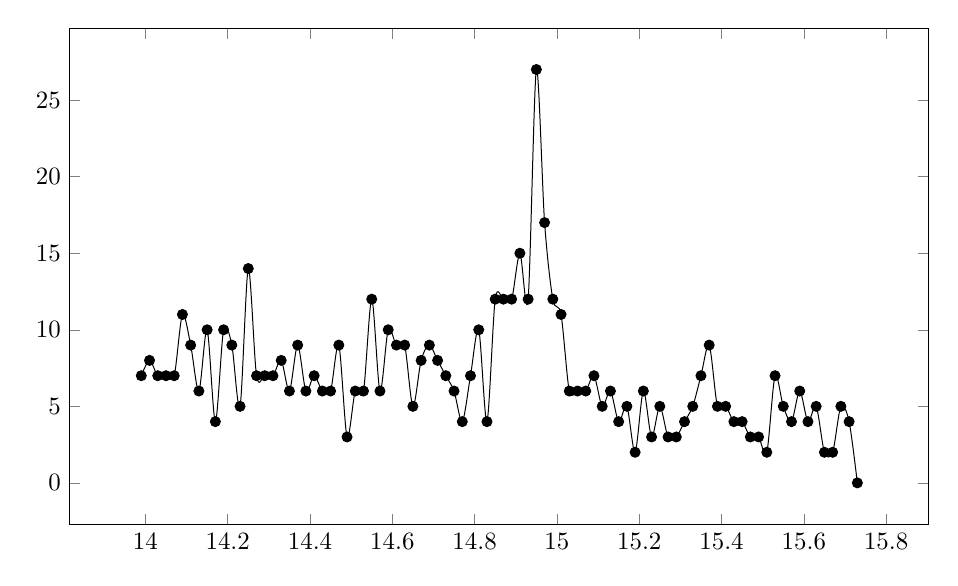
\begin{tikzpicture}[scale=0.9]
	\begin{axis}[
	scale only axis,
	%ymode=log, 
	width=\textwidth, 
	height=7cm
]
	\addplot [smooth,mark=*,black] table {%  plot X versus Y. This is original data.
	X		Y 

 13.990 7
 14.010 8
 14.030 7
 14.050 7
 14.070 7
 14.090 11
 14.110 9
 14.130 6
 14.150 10
 14.170 4
 14.190 10
 14.210 9
 14.230 5
 14.250 14
 14.270 7
 14.290 7
 14.310 7
 14.330 8
 14.350 6
 14.370 9
 14.390 6
 14.410 7
 14.430 6
 14.450 6
 14.470 9
 14.490 3
 14.510 6
 14.530 6
 14.550 12
 14.570 6
 14.590 10
 14.610 9
 14.630 9
 14.650 5
 14.670 8
 14.690 9
 14.710 8
 14.730 7
 14.750 6
 14.770 4
 14.790 7
 14.810 10
 14.830 4
 14.850 12
 14.870 12
 14.890 12
 14.910 15
 14.930 12
 14.950 27
 14.970 17
 14.990 12
 15.010 11
 15.030 6
 15.050 6
 15.070 6
 15.090 7
 15.110 5
 15.130 6
 15.150 4
 15.170 5
 15.190 2
 15.210 6
 15.230 3
 15.250 5
 15.270 3
 15.290 3
 15.310 4
 15.330 5
 15.350 7
 15.370 9
 15.390 5
 15.410 5
 15.430 4
 15.450 4
 15.470 3
 15.490 3
 15.510 2
 15.530 7
 15.550 5
 15.570 4
 15.590 6
 15.610 4
 15.630 5
 15.650 2
 15.670 2
 15.690 5
 15.710 4
 15.730 0
		}
	node[right,red] at (axis cs:38.460,992) {$2\Theta=38.460$}
	node[right,red] at (axis cs:44.700,441) {$2\Theta=44.700$}
	node[right,red] at (axis cs:65.020,1406) {$2\Theta=65.020$}
	node[above,red] at (axis cs:78.100,702) {$2\Theta=78.100$}	
	node[above,red] at (axis cs:85.10,41) {$2\Theta=82.340$};
	\end{axis}
	
\end{tikzpicture}






    	\caption{Scan 3}
	\label{fig:unknownScan}
\end{figure}

\begin{figure}[h!]
	\centering
	\centering
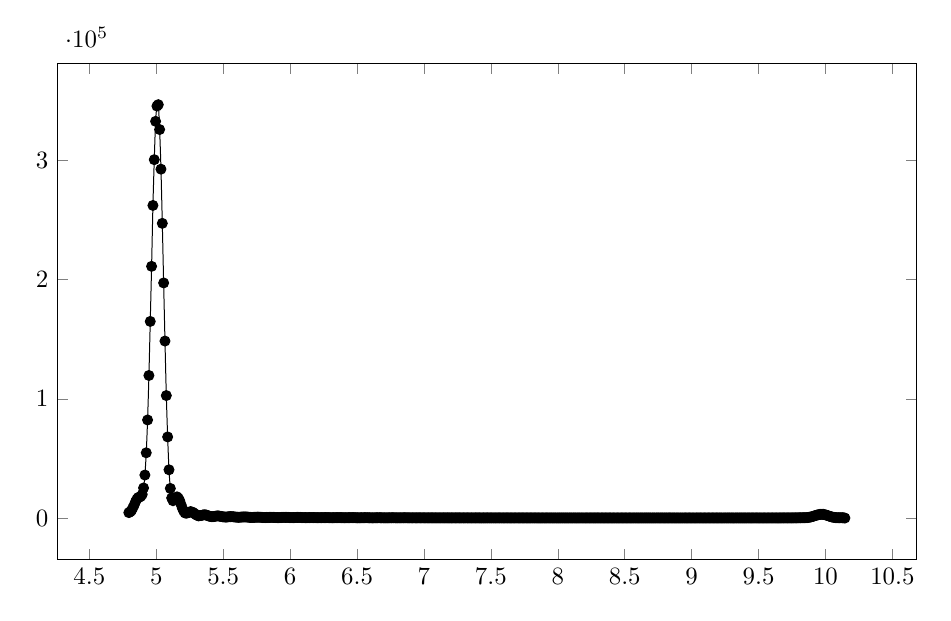
\begin{tikzpicture}[scale=0.9]
	\begin{axis}[
	scale only axis,
	%ymode=log, 
	width=\textwidth, 
	height=7cm
]
	\addplot [smooth,mark=*,black] table {%  plot X versus Y. This is original data.
	X		Y 

  4.795 4556
  4.805 5198
  4.815 6416
  4.825 8593
  4.835 11004
  4.845 13759
  4.855 15826
  4.865 17187
  4.875 17530
  4.885 18252
  4.895 19825
  4.905 25249
  4.915 36100
  4.925 54756
  4.935 82312
  4.945 119647
  4.955 164998
  4.965 211232
  4.975 262349
  4.985 300743
  4.995 332929
  5.005 345744
  5.015 346921
  5.025 326041
  5.035 292789
  5.045 247307
  5.055 197314
  5.065 148533
  5.075 102784
  5.085 68069
  5.095 40481
  5.105 24869
  5.115 16848
  5.125 14520
  5.135 15600
  5.145 16822
  5.155 17796
  5.165 16589
  5.175 14617
  5.185 11342
  5.195 8136
  5.205 5883
  5.215 4238
  5.225 4096
  5.235 4396
  5.245 4789
  5.255 5388
  5.265 5112
  5.275 4679
  5.285 3782
  5.295 2959
  5.305 2294
  5.315 1798
  5.325 1998
  5.335 2144
  5.345 2440
  5.355 2704
  5.365 2704
  5.375 2480
  5.385 2052
  5.395 1521
  5.405 1332
  5.415 1129
  5.425 1211
  5.435 1340
  5.445 1600
  5.455 1789
  5.465 1756
  5.475 1513
  5.485 1340
  5.495 1082
  5.505 967
  5.515 841
  5.525 824
  5.535 999
  5.545 1142
  5.555 1197
  5.565 1170
  5.575 1076
  5.585 912
  5.595 795
  5.605 692
  5.615 620
  5.625 666
  5.635 829
  5.645 858
  5.655 942
  5.665 894
  5.675 876
  5.685 745
  5.695 586
  5.705 529
  5.715 475
  5.725 534
  5.735 600
  5.745 676
  5.755 708
  5.765 686
  5.775 676
  5.785 571
  5.795 458
  5.805 404
  5.815 428
  5.825 462
  5.835 454
  5.845 520
  5.855 557
  5.865 586
  5.875 520
  5.885 471
  5.895 412
  5.905 372
  5.915 372
  5.925 416
  5.935 462
  5.945 520
  5.955 566
  5.965 524
  5.975 552
  5.985 484
  5.995 420
  6.005 376
  6.015 376
  6.025 388
  6.035 404
  6.045 480
  6.055 524
  6.065 524
  6.075 475
  6.085 420
  6.095 357
  6.105 365
  6.115 328
  6.125 310
  6.135 365
  6.145 372
  6.155 384
  6.165 388
  6.175 392
  6.185 372
  6.195 296
  6.205 296
  6.215 286
  6.225 310
  6.235 335
  6.245 328
  6.255 350
  6.265 372
  6.275 369
  6.285 320
  6.295 266
  6.305 266
  6.315 253
  6.325 286
  6.335 292
  6.345 350
  6.355 342
  6.365 331
  6.375 335
  6.385 317
  6.395 292
  6.405 243
  6.415 276
  6.425 269
  6.435 289
  6.445 292
  6.455 324
  6.465 335
  6.475 335
  6.485 299
  6.495 246
  6.505 240
  6.515 219
  6.525 234
  6.535 269
  6.545 243
  6.555 286
  6.565 299
  6.575 292
  6.585 240
  6.595 231
  6.605 219
  6.615 188
  6.625 188
  6.635 234
  6.645 246
  6.655 250
  6.665 269
  6.675 243
  6.685 228
  6.695 213
  6.705 190
  6.715 182
  6.725 199
  6.735 199
  6.745 231
  6.755 228
  6.765 262
  6.775 253
  6.785 222
  6.795 188
  6.805 210
  6.815 199
  6.825 219
  6.835 216
  6.845 225
  6.855 256
  6.865 231
  6.875 199
  6.885 222
  6.895 193
  6.905 174
  6.915 174
  6.925 199
  6.935 169
  6.945 193
  6.955 177
  6.965 210
  6.975 193
  6.985 166
  6.995 199
  7.005 156
  7.015 169
  7.025 149
  7.035 169
  7.045 164
  7.055 182
  7.065 166
  7.075 166
  7.085 156
  7.095 161
  7.105 156
  7.115 146
  7.125 146
  7.135 161
  7.145 159
  7.155 166
  7.165 139
  7.175 154
  7.185 161
  7.195 144
  7.205 137
  7.215 135
  7.225 154
  7.235 137
  7.245 154
  7.255 156
  7.265 137
  7.275 137
  7.285 128
  7.295 149
  7.305 130
  7.315 144
  7.325 139
  7.335 128
  7.345 130
  7.355 128
  7.365 119
  7.375 130
  7.385 142
  7.395 137
  7.405 132
  7.415 121
  7.425 114
  7.435 100
  7.445 130
  7.455 123
  7.465 121
  7.475 132
  7.485 130
  7.495 130
  7.505 108
  7.515 128
  7.525 104
  7.535 106
  7.545 117
  7.555 121
  7.565 123
  7.575 114
  7.585 92
  7.595 108
  7.605 98
  7.615 114
  7.625 110
  7.635 102
  7.645 96
  7.655 102
  7.665 98
  7.675 96
  7.685 119
  7.695 96
  7.705 94
  7.715 92
  7.725 106
  7.735 104
  7.745 96
  7.755 102
  7.765 98
  7.775 102
  7.785 96
  7.795 102
  7.805 108
  7.815 108
  7.825 85
  7.835 104
  7.845 94
  7.855 92
  7.865 83
  7.875 88
  7.885 83
  7.895 86
  7.905 100
  7.915 94
  7.925 104
  7.935 83
  7.945 85
  7.955 94
  7.965 83
  7.975 85
  7.985 71
  7.995 83
  8.005 79
  8.015 76
  8.025 86
  8.035 88
  8.045 85
  8.055 86
  8.065 72
  8.075 86
  8.085 79
  8.095 83
  8.105 85
  8.115 79
  8.125 85
  8.135 100
  8.145 76
  8.155 62
  8.165 86
  8.175 90
  8.185 67
  8.195 72
  8.205 86
  8.215 76
  8.225 79
  8.235 79
  8.245 79
  8.255 88
  8.265 86
  8.275 76
  8.285 94
  8.295 90
  8.305 85
  8.315 71
  8.325 86
  8.335 77
  8.345 79
  8.355 92
  8.365 66
  8.375 71
  8.385 72
  8.395 85
  8.405 71
  8.415 72
  8.425 76
  8.435 76
  8.445 67
  8.455 69
  8.465 76
  8.475 72
  8.485 74
  8.495 72
  8.505 86
  8.515 62
  8.525 71
  8.535 77
  8.545 72
  8.555 66
  8.565 77
  8.575 76
  8.585 62
  8.595 76
  8.605 69
  8.615 72
  8.625 62
  8.635 69
  8.645 76
  8.655 79
  8.665 77
  8.675 76
  8.685 66
  8.695 56
  8.705 66
  8.715 74
  8.725 62
  8.735 72
  8.745 77
  8.755 90
  8.765 66
  8.775 71
  8.785 79
  8.795 71
  8.805 67
  8.815 67
  8.825 62
  8.835 77
  8.845 92
  8.855 79
  8.865 58
  8.875 85
  8.885 64
  8.895 56
  8.905 76
  8.915 66
  8.925 53
  8.935 76
  8.945 81
  8.955 71
  8.965 66
  8.975 77
  8.985 72
  8.995 67
  9.005 69
  9.015 72
  9.025 62
  9.035 72
  9.045 67
  9.055 83
  9.065 77
  9.075 64
  9.085 76
  9.095 72
  9.105 71
  9.115 77
  9.125 72
  9.135 66
  9.145 66
  9.155 86
  9.165 69
  9.175 62
  9.185 77
  9.195 76
  9.205 72
  9.215 71
  9.225 72
  9.235 52
  9.245 72
  9.255 77
  9.265 77
  9.275 79
  9.285 76
  9.295 72
  9.305 69
  9.315 56
  9.325 62
  9.335 86
  9.345 79
  9.355 72
  9.365 76
  9.375 67
  9.385 92
  9.395 71
  9.405 79
  9.415 83
  9.425 74
  9.435 77
  9.445 71
  9.455 85
  9.465 71
  9.475 92
  9.485 79
  9.495 77
  9.505 71
  9.515 69
  9.525 71
  9.535 76
  9.545 81
  9.555 72
  9.565 71
  9.575 90
  9.585 74
  9.595 83
  9.605 104
  9.615 92
  9.625 76
  9.635 86
  9.645 81
  9.655 81
  9.665 88
  9.675 108
  9.685 108
  9.695 123
  9.705 96
  9.715 110
  9.725 128
  9.735 100
  9.745 110
  9.755 137
  9.765 149
  9.775 169
  9.785 154
  9.795 213
  9.805 231
  9.815 225
  9.825 246
  9.835 259
  9.845 289
  9.855 339
  9.865 412
  9.875 571
  9.885 773
  9.895 1037
  9.905 1310
  9.915 1764
  9.925 2079
  9.935 2490
  9.945 2725
  9.955 2992
  9.965 3147
  9.975 3080
  9.985 3047
  9.995 2798
 10.005 2460
 10.015 2162
 10.025 1706
 10.035 1282
 10.045 999
 10.055 740
 10.065 497
 10.075 392
 10.085 276
 10.095 262
 10.105 243
 10.115 262
 10.125 250
 10.135 222
 10.145 0
		}
	node[right,red] at (axis cs:38.460,992) {$2\Theta=38.460$}
	node[right,red] at (axis cs:44.700,441) {$2\Theta=44.700$}
	node[right,red] at (axis cs:65.020,1406) {$2\Theta=65.020$}
	node[above,red] at (axis cs:78.100,702) {$2\Theta=78.100$}	
	node[above,red] at (axis cs:85.10,41) {$2\Theta=82.340$};
	\end{axis}
	
\end{tikzpicture}






    	\caption{Scan 4}
	\label{fig:unknownScan}
\end{figure}

\begin{figure}[h!]
	\centering
	\centering
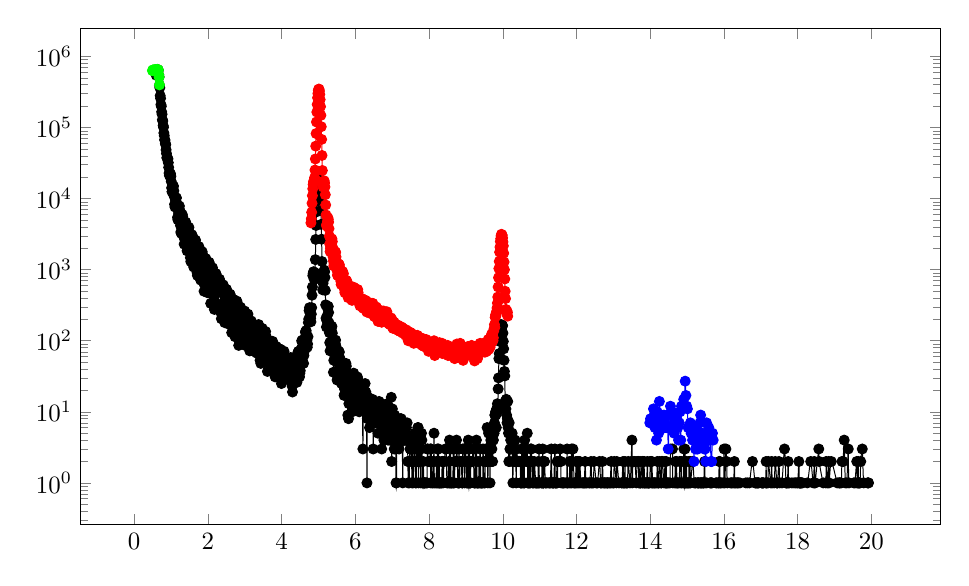
\begin{tikzpicture}[scale=0.9]
	\begin{axis}[
	scale only axis,
	ymode=log, 
	width=\textwidth, 
	height=7cm
]
	\addplot [smooth,mark=*,black] table {%  plot X versus Y. This is original data.
	X		Y 
	
  0.595 545825
  0.605 652541
  0.615 643846
  0.625 655290
  0.635 654805
  0.645 638561
  0.655 639840
  0.665 549526
  0.675 515380
  0.685 394384
  0.695 362524
  0.705 280476
  0.715 257150
  0.725 210497
  0.735 199362
  0.745 166138
  0.755 153899
  0.765 128737
  0.775 123552
  0.785 106602
  0.795 100997
  0.805 83868
  0.815 76895
  0.825 67236
  0.835 66564
  0.845 60123
  0.855 57073
  0.865 48532
  0.875 43139
  0.885 37481
  0.895 37791
  0.905 36787
  0.915 36328
  0.925 32005
  0.935 27490
  0.945 22801
  0.955 21112
  0.965 21550
  0.975 22560
  0.985 22261
  0.995 20564
  1.005 17450
  1.015 14161
  1.025 12477
  1.035 12544
  1.045 13924
  1.055 14860
  1.065 15006
  1.075 12882
  1.085 10733
  1.095 8317
  1.105 7621
  1.115 8172
  1.125 9351
  1.135 10140
  1.145 10262
  1.155 8593
  1.165 7362
  1.175 5432
  1.185 5027
  1.195 5069
  1.205 6288
  1.215 7259
  1.225 7868
  1.235 6856
  1.245 5852
  1.255 4186
  1.265 3387
  1.275 3249
  1.285 4382
  1.295 4998
  1.305 5975
  1.315 5580
  1.325 5112
  1.335 3672
  1.345 2894
  1.355 2285
  1.365 2746
  1.375 3352
  1.385 4476
  1.395 4679
  1.405 4462
  1.415 3516
  1.425 2725
  1.435 1840
  1.445 1866
  1.455 2134
  1.465 3036
  1.475 3446
  1.485 3931
  1.495 3341
  1.505 2756
  1.515 1884
  1.525 1475
  1.535 1303
  1.545 1823
  1.555 2343
  1.565 3102
  1.575 3003
  1.585 2862
  1.595 2200
  1.605 1624
  1.615 1089
  1.625 1102
  1.635 1362
  1.645 1971
  1.655 2314
  1.665 2601
  1.675 2266
  1.685 1892
  1.695 1260
  1.705 912
  1.715 829
  1.725 1211
  1.735 1616
  1.745 2079
  1.755 2116
  1.765 1945
  1.775 1459
  1.785 1116
  1.795 745
  1.805 713
  1.815 870
  1.825 1303
  1.835 1568
  1.845 1789
  1.855 1632
  1.865 1362
  1.875 973
  1.885 650
  1.895 497
  1.905 734
  1.915 1005
  1.925 1391
  1.935 1436
  1.945 1421
  1.955 1253
  1.965 847
  1.975 548
  1.985 475
  1.995 484
  2.005 784
  2.015 1069
  2.025 1274
  2.035 1260
  2.045 1069
  2.055 745
  2.065 534
  2.075 335
  2.085 458
  2.095 562
  2.105 864
  2.115 912
  2.125 1063
  2.135 930
  2.145 778
  2.155 484
  2.165 328
  2.175 276
  2.185 433
  2.195 620
  2.205 795
  2.215 882
  2.225 853
  2.235 718
  2.245 543
  2.255 313
  2.265 276
  2.275 324
  2.285 484
  2.295 650
  2.305 697
  2.315 734
  2.325 655
  2.335 502
  2.345 320
  2.355 246
  2.365 204
  2.375 328
  2.385 471
  2.395 590
  2.405 610
  2.415 610
  2.425 493
  2.435 350
  2.445 250
  2.455 180
  2.465 213
  2.475 324
  2.485 475
  2.495 524
  2.505 529
  2.515 484
  2.525 320
  2.535 219
  2.545 180
  2.555 172
  2.565 240
  2.575 365
  2.585 396
  2.595 454
  2.605 445
  2.615 380
  2.625 282
  2.635 172
  2.645 130
  2.655 169
  2.665 222
  2.675 331
  2.685 376
  2.695 380
  2.705 350
  2.715 256
  2.725 172
  2.735 114
  2.745 128
  2.755 164
  2.765 225
  2.775 303
  2.785 361
  2.795 342
  2.805 269
  2.815 231
  2.825 146
  2.835 86
  2.845 100
  2.855 161
  2.865 213
  2.875 272
  2.885 296
  2.895 266
  2.905 240
  2.915 174
  2.925 128
  2.935 94
  2.945 92
  2.955 151
  2.965 199
  2.975 228
  2.985 222
  2.995 262
  3.005 190
  3.015 154
  3.025 100
  3.035 85
  3.045 117
  3.055 132
  3.065 182
  3.075 225
  3.085 237
  3.095 204
  3.105 154
  3.115 110
  3.125 85
  3.135 72
  3.145 114
  3.155 128
  3.165 174
  3.175 190
  3.185 180
  3.195 149
  3.205 125
  3.215 100
  3.225 72
  3.235 72
  3.245 88
  3.255 125
  3.265 151
  3.275 166
  3.285 164
  3.295 144
  3.305 100
  3.315 72
  3.325 67
  3.335 71
  3.345 90
  3.355 121
  3.365 151
  3.375 169
  3.385 151
  3.395 108
  3.405 86
  3.415 53
  3.425 62
  3.435 48
  3.445 90
  3.455 106
  3.465 130
  3.475 149
  3.485 125
  3.495 90
  3.505 72
  3.515 64
  3.525 53
  3.535 74
  3.545 79
  3.555 117
  3.565 135
  3.575 117
  3.585 98
  3.595 79
  3.605 55
  3.615 37
  3.625 49
  3.635 61
  3.645 72
  3.655 94
  3.665 100
  3.675 86
  3.685 85
  3.695 56
  3.705 56
  3.715 44
  3.725 59
  3.735 61
  3.745 74
  3.755 98
  3.765 88
  3.775 67
  3.785 67
  3.795 50
  3.805 44
  3.815 38
  3.825 31
  3.835 50
  3.845 58
  3.855 83
  3.865 66
  3.875 52
  3.885 46
  3.895 37
  3.905 41
  3.915 35
  3.925 45
  3.935 44
  3.945 59
  3.955 76
  3.965 76
  3.975 64
  3.985 44
  3.995 25
  4.005 38
  4.015 28
  4.025 38
  4.035 53
  4.045 55
  4.055 66
  4.065 71
  4.075 64
  4.085 42
  4.095 32
  4.105 34
  4.115 38
  4.125 38
  4.135 41
  4.145 56
  4.155 50
  4.165 44
  4.175 35
  4.185 31
  4.195 29
  4.205 28
  4.215 28
  4.225 46
  4.235 50
  4.245 58
  4.255 53
  4.265 49
  4.275 53
  4.285 23
  4.295 19
  4.305 26
  4.315 29
  4.325 38
  4.335 46
  4.345 50
  4.355 55
  4.365 46
  4.375 44
  4.385 40
  4.395 28
  4.405 37
  4.415 26
  4.425 45
  4.435 67
  4.445 61
  4.455 71
  4.465 64
  4.475 48
  4.485 31
  4.495 35
  4.505 38
  4.515 53
  4.525 76
  4.535 72
  4.545 100
  4.555 96
  4.565 102
  4.575 77
  4.585 69
  4.595 48
  4.605 62
  4.615 71
  4.625 90
  4.635 110
  4.645 132
  4.655 135
  4.665 139
  4.675 123
  4.685 102
  4.695 81
  4.705 90
  4.715 114
  4.725 180
  4.735 202
  4.745 266
  4.755 292
  4.765 272
  4.775 243
  4.785 207
  4.795 185
  4.805 237
  4.815 292
  4.825 437
  4.835 571
  4.845 824
  4.855 888
  4.865 936
  4.875 853
  4.885 729
  4.895 740
  4.905 906
  4.915 1384
  4.925 2663
  4.935 4186
  4.945 6512
  4.955 9158
  4.965 12122
  4.975 14933
  4.985 17636
  4.995 19600
  5.005 19572
  5.015 19404
  5.025 18010
  5.035 15675
  5.045 12814
  5.055 9663
  5.065 6773
  5.075 4343
  5.085 2683
  5.095 1303
  5.105 773
  5.115 520
  5.125 645
  5.135 829
  5.145 912
  5.155 986
  5.165 930
  5.175 778
  5.185 511
  5.195 320
  5.205 207
  5.215 156
  5.225 193
  5.235 225
  5.245 286
  5.255 306
  5.265 303
  5.275 250
  5.285 180
  5.295 130
  5.305 94
  5.315 72
  5.325 96
  5.335 128
  5.345 151
  5.355 135
  5.365 159
  5.375 128
  5.385 79
  5.395 69
  5.405 36
  5.415 53
  5.425 71
  5.435 79
  5.445 92
  5.455 90
  5.465 102
  5.475 83
  5.485 71
  5.495 50
  5.505 28
  5.515 34
  5.525 30
  5.535 38
  5.545 61
  5.555 71
  5.565 69
  5.575 58
  5.585 35
  5.595 35
  5.605 27
  5.615 30
  5.625 25
  5.635 38
  5.645 38
  5.655 41
  5.665 38
  5.675 44
  5.685 37
  5.695 17
  5.705 21
  5.715 18
  5.725 18
  5.735 27
  5.745 48
  5.755 44
  5.765 36
  5.775 31
  5.785 29
  5.795 9
  5.805 27
  5.815 8
  5.825 13
  5.835 30
  5.845 28
  5.855 29
  5.865 28
  5.875 27
  5.885 18
  5.895 14
  5.905 15
  5.915 10
  5.925 22
  5.935 24
  5.945 28
  5.955 35
  5.965 31
  5.975 24
  5.985 13
  5.995 19
  6.005 12
  6.015 14
  6.025 16
  6.035 20
  6.045 24
  6.055 31
  6.065 29
  6.075 22
  6.085 18
  6.095 14
  6.105 10
  6.115 11
  6.125 17
  6.135 13
  6.145 13
  6.155 22
  6.165 23
  6.175 13
  6.185 14
  6.195 11
  6.205 3
  6.215 12
  6.225 14
  6.235 15
  6.245 18
  6.255 17
  6.265 25
  6.275 16
  6.285 19
  6.295 10
  6.305 10
  6.315 1
  6.325 8
  6.335 15
  6.345 16
  6.355 13
  6.365 11
  6.375 13
  6.385 6
  6.395 11
  6.405 12
  6.415 11
  6.425 14
  6.435 8
  6.445 13
  6.455 13
  6.465 15
  6.475 11
  6.485 3
  6.495 9
  6.505 10
  6.515 8
  6.525 9
  6.535 7
  6.545 10
  6.555 12
  6.565 7
  6.575 12
  6.585 10
  6.595 7
  6.605 7
  6.615 5
  6.625 7
  6.635 10
  6.645 14
  6.655 9
  6.665 8
  6.675 9
  6.685 9
  6.695 13
  6.705 7
  6.715 3
  6.725 9
  6.735 6
  6.745 6
  6.755 7
  6.765 9
  6.775 4
  6.785 6
  6.795 10
  6.805 7
  6.815 5
  6.825 8
  6.835 6
  6.845 5
  6.855 12
  6.865 13
  6.875 10
  6.885 4
  6.895 12
  6.905 8
  6.915 5
  6.925 9
  6.935 4
  6.945 9
  6.955 10
  6.965 6
  6.975 16
  6.985 2
  6.995 4
  7.005 11
  7.015 7
  7.025 5
  7.035 5
  7.045 9
  7.055 3
  7.065 9
  7.075 6
  7.085 4
  7.095 3
  7.105 1
  7.115 1
  7.125 4
  7.135 5
  7.145 8
  7.155 0
  7.165 7
  7.175 7
  7.185 3
  7.195 5
  7.205 5
  7.215 8
  7.225 5
  7.235 4
  7.245 8
  7.255 7
  7.265 7
  7.275 4
  7.285 1
  7.295 4
  7.305 4
  7.315 4
  7.325 6
  7.335 4
  7.345 5
  7.355 4
  7.365 5
  7.375 4
  7.385 6
  7.395 4
  7.405 7
  7.415 4
  7.425 2
  7.435 1
  7.445 2
  7.455 2
  7.465 1
  7.475 4
  7.485 3
  7.495 3
  7.505 4
  7.515 2
  7.525 3
  7.535 1
  7.545 3
  7.555 0
  7.565 1
  7.575 0
  7.585 2
  7.595 4
  7.605 3
  7.615 5
  7.625 2
  7.635 1
  7.645 0
  7.655 1
  7.665 5
  7.675 4
  7.685 2
  7.695 6
  7.705 6
  7.715 1
  7.725 5
  7.735 2
  7.745 2
  7.755 4
  7.765 2
  7.775 1
  7.785 3
  7.795 5
  7.805 4
  7.815 0
  7.825 1
  7.835 1
  7.845 2
  7.855 1
  7.865 1
  7.875 1
  7.885 1
  7.895 1
  7.905 0
  7.915 0
  7.925 0
  7.935 1
  7.945 1
  7.955 3
  7.965 3
  7.975 2
  7.985 0
  7.995 2
  8.005 2
  8.015 2
  8.025 2
  8.035 3
  8.045 1
  8.055 3
  8.065 2
  8.075 0
  8.085 1
  8.095 0
  8.105 1
  8.115 2
  8.125 2
  8.135 5
  8.145 1
  8.155 0
  8.165 0
  8.175 0
  8.185 1
  8.195 0
  8.205 2
  8.215 1
  8.225 3
  8.235 2
  8.245 1
  8.255 3
  8.265 1
  8.275 2
  8.285 1
  8.295 1
  8.305 1
  8.315 0
  8.325 0
  8.335 1
  8.345 1
  8.355 2
  8.365 2
  8.375 0
  8.385 1
  8.395 0
  8.405 2
  8.415 2
  8.425 0
  8.435 0
  8.445 3
  8.455 0
  8.465 3
  8.475 0
  8.485 1
  8.495 0
  8.505 1
  8.515 0
  8.525 0
  8.535 2
  8.545 1
  8.555 4
  8.565 1
  8.575 0
  8.585 3
  8.595 1
  8.605 1
  8.615 1
  8.625 0
  8.635 0
  8.645 1
  8.655 3
  8.665 1
  8.675 3
  8.685 1
  8.695 0
  8.705 2
  8.715 0
  8.725 2
  8.735 2
  8.745 4
  8.755 3
  8.765 2
  8.775 0
  8.785 1
  8.795 1
  8.805 1
  8.815 3
  8.825 1
  8.835 0
  8.845 2
  8.855 0
  8.865 2
  8.875 2
  8.885 0
  8.895 1
  8.905 1
  8.915 3
  8.925 0
  8.935 0
  8.945 3
  8.955 2
  8.965 1
  8.975 0
  8.985 3
  8.995 0
  9.005 2
  9.015 0
  9.025 1
  9.035 1
  9.045 2
  9.055 1
  9.065 4
  9.075 1
  9.085 1
  9.095 3
  9.105 1
  9.115 1
  9.125 1
  9.135 2
  9.145 2
  9.155 0
  9.165 2
  9.175 2
  9.185 0
  9.195 3
  9.205 0
  9.215 0
  9.225 1
  9.235 1
  9.245 1
  9.255 3
  9.265 0
  9.275 1
  9.285 4
  9.295 2
  9.305 1
  9.315 1
  9.325 1
  9.335 0
  9.345 1
  9.355 2
  9.365 0
  9.375 1
  9.385 3
  9.395 0
  9.405 1
  9.415 1
  9.425 1
  9.435 0
  9.445 1
  9.455 1
  9.465 3
  9.475 2
  9.485 0
  9.495 1
  9.505 0
  9.515 1
  9.525 2
  9.535 3
  9.545 2
  9.555 2
  9.565 0
  9.575 6
  9.585 2
  9.595 1
  9.605 2
  9.615 5
  9.625 2
  9.635 2
  9.645 3
  9.655 1
  9.665 6
  9.675 4
  9.685 2
  9.695 0
  9.705 3
  9.715 4
  9.725 2
  9.735 4
  9.745 4
  9.755 5
  9.765 5
  9.775 7
  9.785 9
  9.795 9
  9.805 10
  9.815 9
  9.825 6
  9.835 11
  9.845 10
  9.855 13
  9.865 11
  9.875 21
  9.885 30
  9.895 56
  9.905 66
  9.915 98
  9.925 104
  9.935 146
  9.945 164
  9.955 169
  9.965 161
  9.975 166
  9.985 159
  9.995 164
 10.005 128
 10.015 98
 10.025 77
 10.035 53
 10.045 37
 10.055 32
 10.065 14
 10.075 14
 10.085 11
 10.095 15
 10.105 9
 10.115 7
 10.125 8
 10.135 14
 10.145 6
 10.155 5
 10.165 2
 10.175 7
 10.185 2
 10.195 3
 10.205 3
 10.215 4
 10.225 5
 10.235 3
 10.245 4
 10.255 5
 10.265 2
 10.275 1
 10.285 3
 10.295 2
 10.305 0
 10.315 4
 10.325 2
 10.335 4
 10.345 2
 10.355 2
 10.365 1
 10.375 3
 10.385 0
 10.395 0
 10.405 2
 10.415 0
 10.425 2
 10.435 2
 10.445 0
 10.455 2
 10.465 2
 10.475 2
 10.485 1
 10.495 1
 10.505 1
 10.515 3
 10.525 0
 10.535 1
 10.545 2
 10.555 3
 10.565 2
 10.575 1
 10.585 1
 10.595 4
 10.605 0
 10.615 0
 10.625 0
 10.635 2
 10.645 0
 10.655 0
 10.665 5
 10.675 1
 10.685 2
 10.695 1
 10.705 1
 10.715 0
 10.725 2
 10.735 1
 10.745 1
 10.755 3
 10.765 0
 10.775 3
 10.785 2
 10.795 0
 10.805 1
 10.815 2
 10.825 1
 10.835 0
 10.845 1
 10.855 2
 10.865 0
 10.875 0
 10.885 0
 10.895 1
 10.905 1
 10.915 1
 10.925 0
 10.935 0
 10.945 1
 10.955 1
 10.965 2
 10.975 1
 10.985 3
 10.995 1
 11.005 0
 11.015 0
 11.025 0
 11.035 0
 11.045 1
 11.055 1
 11.065 2
 11.075 1
 11.085 3
 11.095 1
 11.105 1
 11.115 0
 11.125 2
 11.135 2
 11.145 0
 11.155 1
 11.165 1
 11.175 0
 11.185 1
 11.195 0
 11.205 0
 11.215 0
 11.225 1
 11.235 0
 11.245 0
 11.255 0
 11.265 1
 11.275 1
 11.285 0
 11.295 1
 11.305 0
 11.315 3
 11.325 0
 11.335 1
 11.345 0
 11.355 1
 11.365 1
 11.375 1
 11.385 1
 11.395 0
 11.405 0
 11.415 3
 11.425 1
 11.435 1
 11.445 1
 11.455 1
 11.465 0
 11.475 2
 11.485 1
 11.495 2
 11.505 0
 11.515 0
 11.525 2
 11.535 0
 11.545 0
 11.555 3
 11.565 2
 11.575 2
 11.585 1
 11.595 0
 11.605 0
 11.615 0
 11.625 1
 11.635 1
 11.645 1
 11.655 0
 11.665 0
 11.675 0
 11.685 1
 11.695 0
 11.705 0
 11.715 0
 11.725 0
 11.735 1
 11.745 3
 11.755 1
 11.765 1
 11.775 0
 11.785 0
 11.795 0
 11.805 1
 11.815 2
 11.825 0
 11.835 2
 11.845 1
 11.855 0
 11.865 3
 11.875 1
 11.885 0
 11.895 0
 11.905 3
 11.915 0
 11.925 0
 11.935 1
 11.945 1
 11.955 0
 11.965 0
 11.975 1
 11.985 2
 11.995 1
 12.005 0
 12.015 0
 12.025 2
 12.035 1
 12.045 0
 12.055 0
 12.065 2
 12.075 1
 12.085 2
 12.095 0
 12.105 0
 12.115 0
 12.125 1
 12.135 0
 12.145 0
 12.155 0
 12.165 1
 12.175 0
 12.185 1
 12.195 0
 12.205 1
 12.215 1
 12.225 0
 12.235 2
 12.245 0
 12.255 1
 12.265 1
 12.275 0
 12.285 0
 12.295 0
 12.305 0
 12.315 1
 12.325 0
 12.335 0
 12.345 0
 12.355 1
 12.365 1
 12.375 0
 12.385 0
 12.395 2
 12.405 0
 12.415 1
 12.425 1
 12.435 0
 12.445 0
 12.455 0
 12.465 1
 12.475 2
 12.485 0
 12.495 0
 12.505 0
 12.515 0
 12.525 0
 12.535 1
 12.545 0
 12.555 1
 12.565 0
 12.575 1
 12.585 0
 12.595 0
 12.605 0
 12.615 0
 12.625 2
 12.635 0
 12.645 0
 12.655 1
 12.665 1
 12.675 0
 12.685 1
 12.695 0
 12.705 2
 12.715 0
 12.725 1
 12.735 0
 12.745 0
 12.755 1
 12.765 1
 12.775 0
 12.785 1
 12.795 0
 12.805 0
 12.815 0
 12.825 1
 12.835 1
 12.845 1
 12.855 0
 12.865 1
 12.875 0
 12.885 0
 12.895 0
 12.905 1
 12.915 1
 12.925 0
 12.935 0
 12.945 2
 12.955 1
 12.965 0
 12.975 0
 12.985 0
 12.995 1
 13.005 0
 13.015 1
 13.025 2
 13.035 0
 13.045 0
 13.055 0
 13.065 0
 13.075 0
 13.085 1
 13.095 2
 13.105 0
 13.115 0
 13.125 0
 13.135 0
 13.145 0
 13.155 1
 13.165 0
 13.175 0
 13.185 0
 13.195 0
 13.205 0
 13.215 0
 13.225 1
 13.235 1
 13.245 0
 13.255 0
 13.265 2
 13.275 1
 13.285 1
 13.295 0
 13.305 1
 13.315 2
 13.325 1
 13.335 0
 13.345 0
 13.355 1
 13.365 1
 13.375 0
 13.385 1
 13.395 0
 13.405 2
 13.415 0
 13.425 0
 13.435 0
 13.445 0
 13.455 1
 13.465 0
 13.475 0
 13.485 2
 13.495 0
 13.505 4
 13.515 1
 13.525 0
 13.535 2
 13.545 0
 13.555 0
 13.565 0
 13.575 0
 13.585 2
 13.595 0
 13.605 0
 13.615 0
 13.625 1
 13.635 0
 13.645 2
 13.655 0
 13.665 0
 13.675 2
 13.685 0
 13.695 1
 13.705 1
 13.715 0
 13.725 2
 13.735 1
 13.745 1
 13.755 0
 13.765 0
 13.775 0
 13.785 2
 13.795 1
 13.805 1
 13.815 2
 13.825 0
 13.835 2
 13.845 1
 13.855 1
 13.865 1
 13.875 0
 13.885 0
 13.895 1
 13.905 1
 13.915 0
 13.925 2
 13.935 1
 13.945 1
 13.955 1
 13.965 1
 13.975 0
 13.985 1
 13.995 0
 14.005 2
 14.015 0
 14.025 2
 14.035 1
 14.045 2
 14.055 0
 14.065 1
 14.075 1
 14.085 0
 14.095 0
 14.105 1
 14.115 0
 14.125 1
 14.135 1
 14.145 0
 14.155 0
 14.165 0
 14.175 1
 14.185 0
 14.195 2
 14.205 0
 14.215 1
 14.225 1
 14.235 1
 14.245 0
 14.255 2
 14.265 0
 14.275 0
 14.285 0
 14.295 1
 14.305 1
 14.315 2
 14.325 0
 14.335 2
 14.345 0
 14.355 0
 14.365 0
 14.375 1
 14.385 0
 14.395 0
 14.405 2
 14.415 1
 14.425 1
 14.435 2
 14.445 1
 14.455 1
 14.465 0
 14.475 1
 14.485 0
 14.495 0
 14.505 1
 14.515 0
 14.525 0
 14.535 1
 14.545 0
 14.555 3
 14.565 0
 14.575 0
 14.585 0
 14.595 0
 14.605 3
 14.615 1
 14.625 0
 14.635 0
 14.645 0
 14.655 0
 14.665 1
 14.675 0
 14.685 2
 14.695 1
 14.705 0
 14.715 2
 14.725 1
 14.735 1
 14.745 0
 14.755 1
 14.765 0
 14.775 0
 14.785 1
 14.795 0
 14.805 2
 14.815 0
 14.825 2
 14.835 1
 14.845 2
 14.855 1
 14.865 0
 14.875 0
 14.885 0
 14.895 1
 14.905 2
 14.915 3
 14.925 1
 14.935 1
 14.945 3
 14.955 1
 14.965 2
 14.975 1
 14.985 2
 14.995 1
 15.005 0
 15.015 1
 15.025 0
 15.035 1
 15.045 1
 15.055 2
 15.065 2
 15.075 1
 15.085 2
 15.095 1
 15.105 0
 15.115 0
 15.125 0
 15.135 0
 15.145 0
 15.155 2
 15.165 0
 15.175 0
 15.185 0
 15.195 1
 15.205 0
 15.215 0
 15.225 1
 15.235 1
 15.245 0
 15.255 0
 15.265 0
 15.275 0
 15.285 1
 15.295 1
 15.305 0
 15.315 1
 15.325 1
 15.335 0
 15.345 0
 15.355 0
 15.365 1
 15.375 1
 15.385 0
 15.395 1
 15.405 1
 15.415 0
 15.425 0
 15.435 1
 15.445 1
 15.455 1
 15.465 0
 15.475 2
 15.485 0
 15.495 1
 15.505 0
 15.515 0
 15.525 0
 15.535 1
 15.545 0
 15.555 0
 15.565 0
 15.575 0
 15.585 0
 15.595 0
 15.605 0
 15.615 0
 15.625 1
 15.635 1
 15.645 0
 15.655 0
 15.665 1
 15.675 1
 15.685 0
 15.695 0
 15.705 0
 15.715 0
 15.725 0
 15.735 0
 15.745 0
 15.755 0
 15.765 0
 15.775 0
 15.785 1
 15.795 0
 15.805 1
 15.815 0
 15.825 0
 15.835 0
 15.845 1
 15.855 1
 15.865 0
 15.875 2
 15.885 2
 15.895 1
 15.905 1
 15.915 0
 15.925 0
 15.935 0
 15.945 1
 15.955 0
 15.965 0
 15.975 0
 15.985 0
 15.995 1
 16.005 3
 16.015 0
 16.025 1
 16.035 0
 16.045 0
 16.055 3
 16.065 0
 16.075 2
 16.085 0
 16.095 1
 16.105 0
 16.115 0
 16.125 0
 16.135 0
 16.145 0
 16.155 0
 16.165 0
 16.175 1
 16.185 0
 16.195 0
 16.205 1
 16.215 0
 16.225 1
 16.235 0
 16.245 0
 16.255 0
 16.265 1
 16.275 0
 16.285 2
 16.295 1
 16.305 0
 16.315 1
 16.325 0
 16.335 0
 16.345 0
 16.355 1
 16.365 1
 16.375 0
 16.385 0
 16.395 1
 16.405 0
 16.415 0
 16.425 0
 16.435 1
 16.445 0
 16.455 0
 16.465 0
 16.475 0
 16.485 0
 16.495 0
 16.505 0
 16.515 0
 16.525 0
 16.535 0
 16.545 0
 16.555 0
 16.565 0
 16.575 0
 16.585 0
 16.595 1
 16.605 0
 16.615 0
 16.625 0
 16.635 0
 16.645 1
 16.655 0
 16.665 0
 16.675 0
 16.685 0
 16.695 1
 16.705 0
 16.715 0
 16.725 0
 16.735 0
 16.745 0
 16.755 0
 16.765 0
 16.775 2
 16.785 0
 16.795 0
 16.805 0
 16.815 0
 16.825 0
 16.835 0
 16.845 1
 16.855 0
 16.865 1
 16.875 1
 16.885 0
 16.895 0
 16.905 1
 16.915 1
 16.925 0
 16.935 1
 16.945 1
 16.955 0
 16.965 0
 16.975 0
 16.985 0
 16.995 0
 17.005 0
 17.015 0
 17.025 1
 17.035 1
 17.045 1
 17.055 0
 17.065 1
 17.075 1
 17.085 0
 17.095 0
 17.105 0
 17.115 0
 17.125 0
 17.135 1
 17.145 2
 17.155 1
 17.165 1
 17.175 0
 17.185 0
 17.195 1
 17.205 2
 17.215 0
 17.225 0
 17.235 0
 17.245 0
 17.255 0
 17.265 0
 17.275 1
 17.285 0
 17.295 2
 17.305 0
 17.315 1
 17.325 0
 17.335 0
 17.345 0
 17.355 0
 17.365 1
 17.375 0
 17.385 0
 17.395 2
 17.405 0
 17.415 0
 17.425 0
 17.435 1
 17.445 1
 17.455 1
 17.465 0
 17.475 0
 17.485 0
 17.495 2
 17.505 0
 17.515 1
 17.525 0
 17.535 0
 17.545 0
 17.555 0
 17.565 0
 17.575 1
 17.585 0
 17.595 0
 17.605 0
 17.615 0
 17.625 0
 17.635 0
 17.645 3
 17.655 0
 17.665 0
 17.675 0
 17.685 1
 17.695 1
 17.705 1
 17.715 0
 17.725 1
 17.735 0
 17.745 2
 17.755 1
 17.765 0
 17.775 1
 17.785 0
 17.795 0
 17.805 0
 17.815 0
 17.825 0
 17.835 0
 17.845 1
 17.855 0
 17.865 0
 17.875 0
 17.885 0
 17.895 0
 17.905 1
 17.915 0
 17.925 0
 17.935 0
 17.945 1
 17.955 0
 17.965 0
 17.975 0
 17.985 1
 17.995 0
 18.005 1
 18.015 0
 18.025 0
 18.035 2
 18.045 1
 18.055 1
 18.065 1
 18.075 1
 18.085 1
 18.095 1
 18.105 1
 18.115 0
 18.125 0
 18.135 1
 18.145 0
 18.155 0
 18.165 0
 18.175 0
 18.185 0
 18.195 0
 18.205 0
 18.215 0
 18.225 0
 18.235 0
 18.245 0
 18.255 0
 18.265 1
 18.275 0
 18.285 0
 18.295 0
 18.305 0
 18.315 0
 18.325 0
 18.335 0
 18.345 0
 18.355 2
 18.365 0
 18.375 0
 18.385 0
 18.395 0
 18.405 0
 18.415 0
 18.425 1
 18.435 0
 18.445 0
 18.455 2
 18.465 1
 18.475 1
 18.485 0
 18.495 0
 18.505 0
 18.515 0
 18.525 0
 18.535 0
 18.545 0
 18.555 0
 18.565 0
 18.575 3
 18.585 2
 18.595 0
 18.605 0
 18.615 0
 18.625 0
 18.635 0
 18.645 0
 18.655 0
 18.665 0
 18.675 0
 18.685 0
 18.695 1
 18.705 0
 18.715 0
 18.725 0
 18.735 0
 18.745 0
 18.755 0
 18.765 1
 18.775 2
 18.785 0
 18.795 0
 18.805 0
 18.815 1
 18.825 0
 18.835 0
 18.845 2
 18.855 1
 18.865 0
 18.875 0
 18.885 0
 18.895 0
 18.905 0
 18.915 2
 18.925 0
 18.935 0
 18.945 0
 18.955 0
 18.965 0
 18.975 0
 18.985 0
 18.995 0
 19.005 0
 19.015 0
 19.025 0
 19.035 0
 19.045 0
 19.055 0
 19.065 0
 19.075 1
 19.085 0
 19.095 0
 19.105 0
 19.115 0
 19.125 1
 19.135 1
 19.145 0
 19.155 1
 19.165 0
 19.175 0
 19.185 1
 19.195 0
 19.205 2
 19.215 0
 19.225 0
 19.235 2
 19.245 0
 19.255 0
 19.265 4
 19.275 0
 19.285 0
 19.295 1
 19.305 0
 19.315 0
 19.325 0
 19.335 1
 19.345 0
 19.355 0
 19.365 0
 19.375 3
 19.385 0
 19.395 1
 19.405 0
 19.415 0
 19.425 0
 19.435 0
 19.445 0
 19.455 0
 19.465 0
 19.475 0
 19.485 0
 19.495 0
 19.505 0
 19.515 0
 19.525 1
 19.535 0
 19.545 0
 19.555 1
 19.565 0
 19.575 0
 19.585 0
 19.595 0
 19.605 2
 19.615 1
 19.625 0
 19.635 1
 19.645 2
 19.655 1
 19.665 1
 19.675 0
 19.685 1
 19.695 1
 19.705 0
 19.715 2
 19.725 0
 19.735 0
 19.745 0
 19.755 3
 19.765 0
 19.775 0
 19.785 0
 19.795 1
 19.805 0
 19.815 0
 19.825 0
 19.835 0
 19.845 0
 19.855 0
 19.865 0
 19.875 0
 19.885 0
 19.895 1
 19.905 0
 19.915 1
 19.925 1
 19.935 0
 19.945 0
 19.955 0
 19.965 0
 19.975 0
 19.985 0
 19.995 0
	};

	\addplot [smooth,mark=*,green] table {%  plot X versus Y. This is original data.
	X		Y 
  0.495 630436
  0.505 645291
  0.515 632343
  0.525 645452
  0.535 633775
  0.545 647864
  0.555 635528
  0.565 648669
  0.575 633298
  0.585 651572
  0.595 640160
  0.605 653349
  0.615 645612
  0.625 655290
  0.635 655290
  0.645 644488
  0.655 641601
  0.665 555323
  0.675 510939
  0.685 398161
  0.695 0
		};
	
		\addplot [smooth,mark=*,red] table {%  plot X versus Y. This is original data.
	X		Y 

  4.795 4556
  4.805 5198
  4.815 6416
  4.825 8593
  4.835 11004
  4.845 13759
  4.855 15826
  4.865 17187
  4.875 17530
  4.885 18252
  4.895 19825
  4.905 25249
  4.915 36100
  4.925 54756
  4.935 82312
  4.945 119647
  4.955 164998
  4.965 211232
  4.975 262349
  4.985 300743
  4.995 332929
  5.005 345744
  5.015 346921
  5.025 326041
  5.035 292789
  5.045 247307
  5.055 197314
  5.065 148533
  5.075 102784
  5.085 68069
  5.095 40481
  5.105 24869
  5.115 16848
  5.125 14520
  5.135 15600
  5.145 16822
  5.155 17796
  5.165 16589
  5.175 14617
  5.185 11342
  5.195 8136
  5.205 5883
  5.215 4238
  5.225 4096
  5.235 4396
  5.245 4789
  5.255 5388
  5.265 5112
  5.275 4679
  5.285 3782
  5.295 2959
  5.305 2294
  5.315 1798
  5.325 1998
  5.335 2144
  5.345 2440
  5.355 2704
  5.365 2704
  5.375 2480
  5.385 2052
  5.395 1521
  5.405 1332
  5.415 1129
  5.425 1211
  5.435 1340
  5.445 1600
  5.455 1789
  5.465 1756
  5.475 1513
  5.485 1340
  5.495 1082
  5.505 967
  5.515 841
  5.525 824
  5.535 999
  5.545 1142
  5.555 1197
  5.565 1170
  5.575 1076
  5.585 912
  5.595 795
  5.605 692
  5.615 620
  5.625 666
  5.635 829
  5.645 858
  5.655 942
  5.665 894
  5.675 876
  5.685 745
  5.695 586
  5.705 529
  5.715 475
  5.725 534
  5.735 600
  5.745 676
  5.755 708
  5.765 686
  5.775 676
  5.785 571
  5.795 458
  5.805 404
  5.815 428
  5.825 462
  5.835 454
  5.845 520
  5.855 557
  5.865 586
  5.875 520
  5.885 471
  5.895 412
  5.905 372
  5.915 372
  5.925 416
  5.935 462
  5.945 520
  5.955 566
  5.965 524
  5.975 552
  5.985 484
  5.995 420
  6.005 376
  6.015 376
  6.025 388
  6.035 404
  6.045 480
  6.055 524
  6.065 524
  6.075 475
  6.085 420
  6.095 357
  6.105 365
  6.115 328
  6.125 310
  6.135 365
  6.145 372
  6.155 384
  6.165 388
  6.175 392
  6.185 372
  6.195 296
  6.205 296
  6.215 286
  6.225 310
  6.235 335
  6.245 328
  6.255 350
  6.265 372
  6.275 369
  6.285 320
  6.295 266
  6.305 266
  6.315 253
  6.325 286
  6.335 292
  6.345 350
  6.355 342
  6.365 331
  6.375 335
  6.385 317
  6.395 292
  6.405 243
  6.415 276
  6.425 269
  6.435 289
  6.445 292
  6.455 324
  6.465 335
  6.475 335
  6.485 299
  6.495 246
  6.505 240
  6.515 219
  6.525 234
  6.535 269
  6.545 243
  6.555 286
  6.565 299
  6.575 292
  6.585 240
  6.595 231
  6.605 219
  6.615 188
  6.625 188
  6.635 234
  6.645 246
  6.655 250
  6.665 269
  6.675 243
  6.685 228
  6.695 213
  6.705 190
  6.715 182
  6.725 199
  6.735 199
  6.745 231
  6.755 228
  6.765 262
  6.775 253
  6.785 222
  6.795 188
  6.805 210
  6.815 199
  6.825 219
  6.835 216
  6.845 225
  6.855 256
  6.865 231
  6.875 199
  6.885 222
  6.895 193
  6.905 174
  6.915 174
  6.925 199
  6.935 169
  6.945 193
  6.955 177
  6.965 210
  6.975 193
  6.985 166
  6.995 199
  7.005 156
  7.015 169
  7.025 149
  7.035 169
  7.045 164
  7.055 182
  7.065 166
  7.075 166
  7.085 156
  7.095 161
  7.105 156
  7.115 146
  7.125 146
  7.135 161
  7.145 159
  7.155 166
  7.165 139
  7.175 154
  7.185 161
  7.195 144
  7.205 137
  7.215 135
  7.225 154
  7.235 137
  7.245 154
  7.255 156
  7.265 137
  7.275 137
  7.285 128
  7.295 149
  7.305 130
  7.315 144
  7.325 139
  7.335 128
  7.345 130
  7.355 128
  7.365 119
  7.375 130
  7.385 142
  7.395 137
  7.405 132
  7.415 121
  7.425 114
  7.435 100
  7.445 130
  7.455 123
  7.465 121
  7.475 132
  7.485 130
  7.495 130
  7.505 108
  7.515 128
  7.525 104
  7.535 106
  7.545 117
  7.555 121
  7.565 123
  7.575 114
  7.585 92
  7.595 108
  7.605 98
  7.615 114
  7.625 110
  7.635 102
  7.645 96
  7.655 102
  7.665 98
  7.675 96
  7.685 119
  7.695 96
  7.705 94
  7.715 92
  7.725 106
  7.735 104
  7.745 96
  7.755 102
  7.765 98
  7.775 102
  7.785 96
  7.795 102
  7.805 108
  7.815 108
  7.825 85
  7.835 104
  7.845 94
  7.855 92
  7.865 83
  7.875 88
  7.885 83
  7.895 86
  7.905 100
  7.915 94
  7.925 104
  7.935 83
  7.945 85
  7.955 94
  7.965 83
  7.975 85
  7.985 71
  7.995 83
  8.005 79
  8.015 76
  8.025 86
  8.035 88
  8.045 85
  8.055 86
  8.065 72
  8.075 86
  8.085 79
  8.095 83
  8.105 85
  8.115 79
  8.125 85
  8.135 100
  8.145 76
  8.155 62
  8.165 86
  8.175 90
  8.185 67
  8.195 72
  8.205 86
  8.215 76
  8.225 79
  8.235 79
  8.245 79
  8.255 88
  8.265 86
  8.275 76
  8.285 94
  8.295 90
  8.305 85
  8.315 71
  8.325 86
  8.335 77
  8.345 79
  8.355 92
  8.365 66
  8.375 71
  8.385 72
  8.395 85
  8.405 71
  8.415 72
  8.425 76
  8.435 76
  8.445 67
  8.455 69
  8.465 76
  8.475 72
  8.485 74
  8.495 72
  8.505 86
  8.515 62
  8.525 71
  8.535 77
  8.545 72
  8.555 66
  8.565 77
  8.575 76
  8.585 62
  8.595 76
  8.605 69
  8.615 72
  8.625 62
  8.635 69
  8.645 76
  8.655 79
  8.665 77
  8.675 76
  8.685 66
  8.695 56
  8.705 66
  8.715 74
  8.725 62
  8.735 72
  8.745 77
  8.755 90
  8.765 66
  8.775 71
  8.785 79
  8.795 71
  8.805 67
  8.815 67
  8.825 62
  8.835 77
  8.845 92
  8.855 79
  8.865 58
  8.875 85
  8.885 64
  8.895 56
  8.905 76
  8.915 66
  8.925 53
  8.935 76
  8.945 81
  8.955 71
  8.965 66
  8.975 77
  8.985 72
  8.995 67
  9.005 69
  9.015 72
  9.025 62
  9.035 72
  9.045 67
  9.055 83
  9.065 77
  9.075 64
  9.085 76
  9.095 72
  9.105 71
  9.115 77
  9.125 72
  9.135 66
  9.145 66
  9.155 86
  9.165 69
  9.175 62
  9.185 77
  9.195 76
  9.205 72
  9.215 71
  9.225 72
  9.235 52
  9.245 72
  9.255 77
  9.265 77
  9.275 79
  9.285 76
  9.295 72
  9.305 69
  9.315 56
  9.325 62
  9.335 86
  9.345 79
  9.355 72
  9.365 76
  9.375 67
  9.385 92
  9.395 71
  9.405 79
  9.415 83
  9.425 74
  9.435 77
  9.445 71
  9.455 85
  9.465 71
  9.475 92
  9.485 79
  9.495 77
  9.505 71
  9.515 69
  9.525 71
  9.535 76
  9.545 81
  9.555 72
  9.565 71
  9.575 90
  9.585 74
  9.595 83
  9.605 104
  9.615 92
  9.625 76
  9.635 86
  9.645 81
  9.655 81
  9.665 88
  9.675 108
  9.685 108
  9.695 123
  9.705 96
  9.715 110
  9.725 128
  9.735 100
  9.745 110
  9.755 137
  9.765 149
  9.775 169
  9.785 154
  9.795 213
  9.805 231
  9.815 225
  9.825 246
  9.835 259
  9.845 289
  9.855 339
  9.865 412
  9.875 571
  9.885 773
  9.895 1037
  9.905 1310
  9.915 1764
  9.925 2079
  9.935 2490
  9.945 2725
  9.955 2992
  9.965 3147
  9.975 3080
  9.985 3047
  9.995 2798
 10.005 2460
 10.015 2162
 10.025 1706
 10.035 1282
 10.045 999
 10.055 740
 10.065 497
 10.075 392
 10.085 276
 10.095 262
 10.105 243
 10.115 262
 10.125 250
 10.135 222
 10.145 0
		};
	
		\addplot [smooth,mark=*,blue] table {%  plot X versus Y. This is original data.
	X		Y 

 13.990 7
 14.010 8
 14.030 7
 14.050 7
 14.070 7
 14.090 11
 14.110 9
 14.130 6
 14.150 10
 14.170 4
 14.190 10
 14.210 9
 14.230 5
 14.250 14
 14.270 7
 14.290 7
 14.310 7
 14.330 8
 14.350 6
 14.370 9
 14.390 6
 14.410 7
 14.430 6
 14.450 6
 14.470 9
 14.490 3
 14.510 6
 14.530 6
 14.550 12
 14.570 6
 14.590 10
 14.610 9
 14.630 9
 14.650 5
 14.670 8
 14.690 9
 14.710 8
 14.730 7
 14.750 6
 14.770 4
 14.790 7
 14.810 10
 14.830 4
 14.850 12
 14.870 12
 14.890 12
 14.910 15
 14.930 12
 14.950 27
 14.970 17
 14.990 12
 15.010 11
 15.030 6
 15.050 6
 15.070 6
 15.090 7
 15.110 5
 15.130 6
 15.150 4
 15.170 5
 15.190 2
 15.210 6
 15.230 3
 15.250 5
 15.270 3
 15.290 3
 15.310 4
 15.330 5
 15.350 7
 15.370 9
 15.390 5
 15.410 5
 15.430 4
 15.450 4
 15.470 3
 15.490 3
 15.510 2
 15.530 7
 15.550 5
 15.570 4
 15.590 6
 15.610 4
 15.630 5
 15.650 2
 15.670 2
 15.690 5
 15.710 4
 15.730 0
		};

	\end{axis}
	
\end{tikzpicture}






    	\caption{all scans together}
	\label{fig:unknownScan}
\end{figure}